\section{Appendix Carnot Cycle from Unruh--Landauer}
\label{sec:carnot}

The Carnot cycle developed here is evaluated at the saturation 
frequency $\omega_{\mathrm{sat}} = a\ln 2/c$ of 
Section~\ref{sec:saturation}, the unique frequency 
at which a single photon deposits exactly one bit 
of Bremermann channel capacity per Rindler period. 
At this frequency the Unruh temperature 
$k_BT_H = \hbar a/2\pi c$ and the photon energy 
$\hbar\omega_{\mathrm{sat}} = \hbar a\ln 2/c$ are 
related by
%
\begin{equation}
    k_BT_H = \frac{\hbar\omega_{\mathrm{sat}}}{\ln 2},
    \label{eq:TH_sat}
\end{equation}
%
which is $k_BT_H \sim \hbar\omega_{\mathrm{sat}}$ 
up to the factor $1/\ln 2 \approx 1.44$, the 
nats-to-bits conversion. This factor has a precise 
meaning in the present framework: it is the ratio 
between the natural information unit of the Unruh 
thermal distribution (nats, set by $e$) and the 
binary unit of the helicity outcome (bits, set by 
$\ln 2$). Throughout this section we absorb this 
factor into the order-of-magnitude identification
%
\begin{equation}
    k_BT_H \sim \hbar\omega_{\mathrm{sat}},
    \label{eq:TH_order}
\end{equation}
%
consistent with the heuristic character of the 
Schwarzschild radius and surface gravity 
derivations of Section~\ref{sec:heuristics}, 
where numerical prefactors of the same order 
appear for the same reason. The precise 
coefficient is recovered by working in nats 
throughout, in which case $\ln 2 \to 1$ and 
equation~\eqref{eq:TH_sat} becomes exact. The 
six equivalent conditions of the upcoming
Proposition~\ref{prop:eft} all reduce to 
$\omega = \omega_{\mathrm{sat}}$ at the horizon, 
so evaluating the cycle at this frequency is not 
an additional assumption but the condition that 
the EFT, which we will explore in the next section, is at its natural boundary.

The Carnot cycle developed here is formulated at the level of 
individual non-thermal microstates, and this is the point. 
Reversibility is a feature of the microstate description: in a 
coarse-grained thermal treatment individual microstates are 
inaccessible and the cycle could not be run explicitly. Temperature 
appears in this section not as a primitive imported from the Rindler 
description but as a derived label on each leg of the cycle, 
consistent with the non-thermal Minkowski vantage point maintained 
throughout. The Carnot efficiency bound and the Unruh--Landauer 
bound will emerge as the same inequality viewed from opposite sides 
of this microstate-level construction, closing the loop opened in 
Section~\ref{sec:heuristics}.

We consider in this section the case where $\mathcal{L}$ and $\mathcal{R}$ are moving mirrors being accelerated with an outward thrust from our past bilocal source $\mathcal{P}$ emission, see Figure \ref{carnot}. We complete our bilocal microstate absorption example by reflecting and emitting the photons off of the mirrors.


This reflects the energy back to the future sink 
$\mathcal{F}$, located at $(t,z) = (1,0)$, which is 
the PCT image of $\mathcal{P}$ under the combined 
time-reversal and parity operation that swaps past 
and future wedges. $\mathcal{F}$ plays the role of 
a final absorber, receiving the reflected photons 
and resetting the field state; its existence is 
required by the reversibility of the ideal mirror 
cycle and by the PCT symmetry of the bilocal 
construction. The reflection is reversible in the 
sense that the mirrors do not retain a persistent 
copy of the information that they temporarily store.

The mirrors are ideal, in the sense that they do not retain a persistent copy of the information that they temporarily store; they forget and emit. It is this reversibility that allows us to construct a example of a Carnot cycle at the level of microstates. The working system is the photon–mirror interaction degree of freedom; the Rindler wedge defines the thermal reservoirs, and the mirror trajectory defines the work parameter.

\begin{figure}[h]
\centering
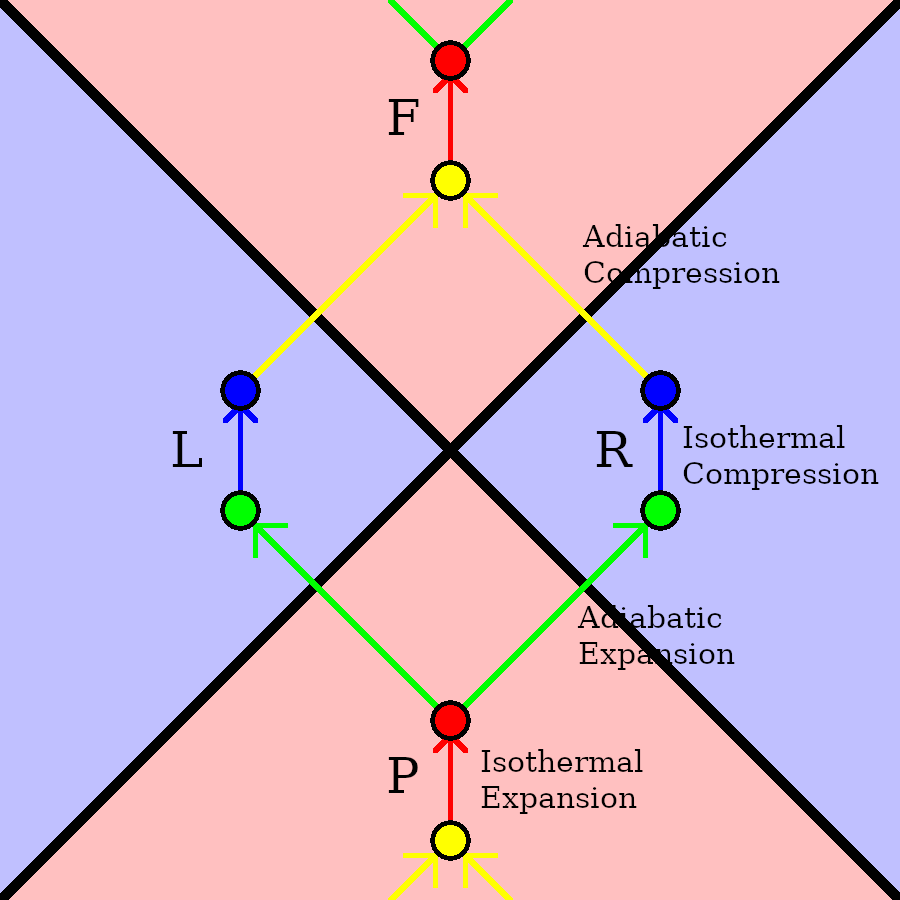
\includegraphics[scale=0.75]{carnot.png}
\captionsetup{width=0.7\textwidth}
\caption{Carnot Cycle: Past ($\mathcal{P}$) bilocal source emits entangled pair with one leg hitting a moving mirror in the right wedge ($\mathcal{R}$). Reflection focuses to a future sink ($\mathcal{F}$). A similar balancing situation exists in the left wedge.}
\label{carnot}
\end{figure}

Consider the point of view of the right Rindler observer $\mathcal{R}$ who sees the event horizon as a thermal object.
The Rindler horizon plays the role of the hot reservoir 
at the Unruh temperature $T_H = \hbar a/2\pi k_B c$, 
consistent with the standard identification of the 
horizon as a thermal object and its connection to the 
generalised second law~\cite{unruh1982acceleration}.
The Rindler wedge interior, where the mirror operates, 
is taken as the cold reservoir at temperature $T_C$. The 
identification of $T_C$ with the Landauer erasure temperature 
of the mirror is an ansatz of the present construction; its 
precise value determines the Carnot efficiency $\eta = 1 - T_C/T_H$.

\begin{itemize} 
\item {\bf Isothermal Expansion:} The bilocal source prepares an entangled photon pair in the basis that $\mathcal{R}$ measures in ($H_+/H_-$ see section \ref{sec:erepr}). In this basis, the Shannon entropy of the Rindler outcome distribution increases from 0 to 1 bit, reflecting the transition from a deterministic prior state to a maximally uncertain Bell state induced by the bilocal entanglement structure,
  , i.e.\ the inverse of the PVM projection 
of Section~\ref{sec:pvm_localization}: 
the isothermal expansion runs the projection 
backward, from a sharp microstate to the 
full superposition; notionally ``drawing some heat from the environment $\mathcal{P}$''.
\item {\bf Adiabatic Expansion:} This corresponds to the crossing over the past Rindler horizon from hot to cold, the absorption of the photon by the mirror.
\item {\bf Isothermal Compression:} This corresponds to controlled 
erasure of the detector's stored bit during the re-emission of the photon 
by the mirror.
This is where the Landauer cost is 
paid~\cite{landauer1961irreversibility, 
bennett1982thermodynamics}: Bennett showed that 
measurement can in principle be performed 
reversibly; it is the erasure of the stored bit 
at re-emission that necessarily dissipates energy, 
at minimum $k_BT_C \ln 2$ into the cold reservoir.
\item {\bf Adiabatic Compression:} This corresponds to the crossing over the future Rindler horizon from cold to hot, the absorption of the future sink $\mathcal{F}$ and reseting of the state to an eigenstate of $H_+$ or $H_-$, zero bits of Shannon entropy. 
\end{itemize}


\subsection{Shannon Entropy, QBism, and 
Wigner's Friend}

The entropy variation in the isothermal legs should be 
understood as Shannon entropy associated with 
measurement outcomes in a fixed operational basis, 
rather than the von Neumann entropy of the global 
quantum state, which remains pure throughout. This 
distinction has a precise foundation. The four-observer 
structure $\mathcal{P}$--$\mathcal{R}$--$\mathcal{L}$--$\mathcal{F}$ 
is a gravitational realisation of the Wigner's friend 
scenario~\cite{brukner2018no}: $\mathcal{P}$ 
prepares the Bell state (Wigner's role), 
$\mathcal{R}$ and $\mathcal{L}$ each measure it 
(the friends' roles), and the question of when 
``collapse'' occurred is observer-relative. From 
$\mathcal{R}$'s perspective, the state collapsed 
upon photon absorption; from the full Minkowski 
perspective, the global state remained pure 
throughout. These descriptions are not contradictory 
but complementary.

The QBist framework~\cite{fuchs2014introducing} resolves 
this cleanly, and is the natural home of the present 
construction. In QBism, quantum states encode an 
agent's beliefs rather than objective microstate 
facts; the correlations between agents' outcomes 
are objectively real and correctly predicted by the 
Bell state structure, but no single agent holds the 
``true'' global state. Each observer's Shannon 
entropy, the uncertainty in their helicity 
outcome prior to measurement, is valid relative 
to them. The Carnot cycle is therefore formulated 
relative to $\mathcal{R}$: its Shannon entropy 
increases from zero to one bit on the isothermal 
expansion leg, decreases on the isothermal 
compression leg, and the area of the cycle in 
$T$-$H$ space is the work extracted, all defined 
by $\mathcal{R}$'s operational measurement basis.

No decoherence assumption is required; Shannon 
entropy here is defined over the classical outcome 
distribution induced by a fixed measurement basis 
(the Rindler detector algebra), independent of the 
unitary evolution of the global state. The objectivity 
of the Bekenstein--Hawking area count is not in 
tension with the observer-relativity of the 
individual microstate: the area increment 
$\Delta A = 8\pi G\hbar\omega$ is a covariant 
physical event, while the assignment of that event 
to a particular observer's measurement record is 
relational. Thermodynamic entropy, in this reading, 
is the classical face of quantum observer-relativity: 
it measures what a given agent does not yet know, 
and its increase under measurement is the same 
process as the Bayesian update arrow of 
Figure~\ref{fig:diagram}, now with a thermodynamic 
label attached.

The interpretational position underlying the 
construction deserves to be stated explicitly. 
Quantum information is treated here as an 
extension of classical information rather than 
a replacement for it. A Hilbert space of 
dimension $2^n$ for $n$ qubits has the same 
dimensional structure as the probability space 
of $n$ classical bits: the statement that two 
coins are correlated as HH or TT but never HT 
or TH already requires a $2^2$-dimensional 
description, and the Bell 
state~\eqref{eq:microstate_vec} is the quantum 
analog of exactly such a classical correlation, 
with probability amplitudes replacing 
probabilities. Quantum observation is 
correspondingly the quantum analog of Bayesian 
conditionalization: the PVM projection updates 
an agent's probability assignment upon receipt 
of a classical outcome. No commitment to a 
specific ontology is required to say this.

The stand the construction takes enters 
precisely at the PVM rule: each handoff event 
is a projective measurement, and its outcome,
the helicity eigenvalue, the spatial bit, 
is recorded in the observer's matter-memory as 
a persistent classical fact. Memory is what 
grounds an observer in their particular 
sequence of outcomes. To interfere with an 
observer who recorded $H_+$ would require 
erasing that record; without erasure, the 
memory distinguishes the two outcomes and no 
interference is possible. The Carnot cycle's 
isothermal compression step is the precise 
physical implementation of this: the mirror 
forgets the bit it learned, paying the Landauer 
cost $k_BT_C\ln 2$. The ideal mirror limit 
$T_C\to 0$ is the limit of perfect forgetting 
at zero thermodynamic cost; the condition 
$T_C>0$ is the condition that some memory 
persists and some coherence is permanently 
lost. The paper does not resolve whether 
perfect forgetting constitutes a transition 
between Everettian branches or a local reset 
of the field state; it shows that the 
thermodynamic cost of forgetting is real and 
precisely calculable, and that the spatial bit, 
the PVM, the matter-memory, and the Landauer 
erasure are the vocabulary in which that 
question must eventually be posed.

\subsection{Work and Efficiency}

The thermodynamic state space of the cycle is parameterised 
by temperature $T$ and Shannon entropy $H$. The two 
isothermal legs operate at $T_H$ and $T_C$ respectively, 
and the entropy change per cycle is exactly one bit:
%
\begin{equation}
\Delta H = \ln 2 \quad \text{(one binary helicity outcome)},
\end{equation}
%
so the work extracted per cycle is the area of the rectangle 
in $T$-$H$ space:
%
\begin{equation}
W = (T_H - T_C)\,\Delta H = (T_H - T_C)\ln 2.
\label{eq:carnot_work}
\end{equation}
%
The work done on the mirror by absorbing one photon of energy 
$\hbar\omega$ is the radiation pressure impulse $\Delta p = 
\hbar\omega/c$, which is responsible for the mirror's 
acceleration into the Rindler wedge. This identifies the hot 
reservoir temperature via
%
\begin{equation}
k_BT_H = \hbar\omega,
\label{eq:TH}
\end{equation}
%
the energy of one photon sets the Unruh temperature of the 
horizon. The Carnot efficiency bound $W \leq T_H\Delta H$ 
then gives
%
\begin{equation}
W \leq \hbar\omega\ln 2 = \frac{\hbar a \ln 2}{2\pi c},
\label{eq:carnot_bound}
\end{equation}
%
where in the last step we used $k_BT_H = \hbar a/2\pi k_Bc$ 
from the Unruh temperature. This is precisely the 
Unruh--Landauer bound~\eqref{eq:UL} at $\Delta H = \ln 2$:
%
\begin{equation}
\boxed{W \leq \frac{\hbar a}{2\pi c}\Delta H 
\iff \Delta E \geq \frac{\hbar a}{2\pi c}\Delta H.}
\label{eq:carnot_UL}
\end{equation}
%
The Carnot efficiency bound for this cycle and the 
Unruh--Landauer bound are therefore the same inequality, 
approached from opposite directions: the Carnot bound is a 
statement about the maximum work extractable from the thermal 
gradient between the horizon and the wedge interior, while 
the Unruh--Landauer bound is a statement about the minimum 
energy cost of acquiring one bit at that horizon. Their 
equivalence identifies the Rindler horizon as a Carnot engine 
operating at the Unruh temperature, with quantum measurement 
as the working substance and the classical bit as the 
thermodynamic output.

The classical precursor to this equivalence is the 
Geroch process~\cite{bekenstein}: a box of radiation 
lowered toward a black hole on a string extracts work 
until, at the horizon, the box carries zero energy 
from the perspective of an observer at infinity. 
Bekenstein showed that dropping the box in must 
increase the black hole's area, establishing a maximum 
efficiency for work extraction that saves the second 
law~\cite{bekenstein}. Our mirror plays the role of 
the box, the measurement impulse plays the role of 
the string tension, and the Unruh--Landauer bound is 
Bekenstein's efficiency constraint expressed in the 
language of information acquisition at the Rindler 
horizon. The two bounds are not merely analogous; 
they are the same inequality, with the Geroch process 
as its classical limit and the Carnot cycle here as 
its microstate realisation.

The cold reservoir temperature $T_C$ is the Landauer 
temperature associated with isolating the mirror from 
its local re-emission environment, while $T_H$ is the 
Landauer temperature associated with isolating the entire 
Rindler wedge from the global Minkowski vacuum. The two 
temperatures correspond to two levels of coarse-graining: 
$T_H$ traces out the opposite wedge at the Rindler horizon, 
while $T_C$ traces out only the mirror's local photon field 
at the scale of the mirror interaction. The temperature 
gradient $T_H > T_C$ is therefore a gradient between 
two scales of isolation, and the Carnot efficiency 
$\eta = 1 - T_C/T_H$ measures how much of the global 
thermal gradient is captured by the local mirror 
interaction. In the limit $T_C \to 0$ the mirror's 
local environment is fully decoupled and the cycle 
extracts maximum work; in the limit $T_C \to T_H$ 
the two scales of isolation coincide and the cycle 
is in hydrostatic equilibrium with no net work extracted.


The efficiency $\eta = 1 - T_C/T_H$ is 
maximised in the limit $T_C \to 0$, which corresponds to 
perfect erasure at zero thermodynamic cost, the ideal 
mirror limit. Any residual $T_C > 0$ reflects irreversibility 
in the mirror's erasure process, consistent with Landauer's 
principle applied to the re-emission step.
